\chapter{システムの線形性とその同定}
対象とするシステムのモデルを作成することで,直接力を測定することなく他のセンサの値から力を推定することが可能である.
前章で導出した物理モデルにおいて未知パラメータを同定すればモデルの構築は可能である.
しかし,バルクや粘性項などのパラメータは温度や圧力などに依存しており,これらのパラメータを正確にしること,そしてすべてのパラメータを同定してモデルを組み上げることは現実的には難しい.

そこで本章ではシステム同定を用いて油圧システムのモデルの構築を行う.
システム同定にあたっては入出力関係を見て同定を行うため,未知パラメータを一つ一つ同定することなくモデルの作成を行うことが可能である.
そこで,バルブへの電圧入力からシリンダ先端の位置及び先端で発生する力までのモデルを,システム同定を用いて導出する.
力の同定ではシリンダ先端を固定した状態で同定をする.
位置の同定にあたっては無負荷状態で行う.
%同定にあたってはシステムの周波数応答を調べて特徴を把握したのちに最小自乗法によるモデルの同定,およびM系列を用いた同定を行いそれぞれを比較する.
\section{実験機とその構成}
本研究で使用する油圧システムの実験装置を\figname\ref{fig:}に示す.
本装置は片ロッドの油圧シリンダ,ギヤポンプ,サーボバルブなどにより構成されており,シリンダにはワイヤー式エンコーダとロードセルが取り付けてある.
また,圧力センサをサーボバルブのAポートおよびBポート,そしてシリンダのヘッド側とロッド側の入り口の計4箇所に取り付けてある.

コントローラ側はPC及びAD/DA変換器やカウンタで構成されており,実験装置に取り付けてあるセンサからの値の取得及びサーボバルブへの入力を行うことができる.
センサ値の処理やサーボバルブへの入力をするための制御アルゴリズムはPC上でMATLAB/Simulinkを用いて組んでいる.
本装置に用いている各部品の諸元をTable~\ref{tab:}にまとめる.
また,システムの伝達経路の全体像は\figname\ref{fig:}のようになる.
\begin{table}[t]
    \centering
    \begin{tabular}{cccc}
        \hline
        Name & Maker & Model Number & Property\\ \hline \hline
        Servo Valve & nachi & J869-1000A & --- \\
        Hydraulic Cylinder & SMC & CHN-25-250 &     \begin{tabular}{l}internel diameter: \SI{25}{mm} \\ rod diameter: \SI{12}{mm}\end{tabular}\\
        Gear Pump & --- & --- &rated power\SI{7}{Mpa},\SI{2}{l/min} \\\hline
        Load Cell & KYOWA & LUK-A-10kN & ---\\
        Pressure Sensor & KEYENCE & GP-M250? & --- \\
        Encoder & Micro Tech Labolatory & & --- \\ \hline
    PC & mouse computer & --- & \begin{tabular}{l}cpu:i7-7900K \\ gpu:\\OS:windows 10 education\end{tabular} \\
    \begin{tabular}{l}AD/DA Converter \\ C8ounter\end{tabular}
    & Speedgoat & Speedgoat & --- \\ 
    MATLAB/Simulink & MathWorks & 2018b & --- \\ \hline \hline
    \end{tabular}
    \caption{Experiment System Configuration}
\end{table}


\section{先端で発生する力までの線形性とモデルの同定}
バルブへの入力から先端で発生する力までのシステム同定にあたり,\figname\ref{fig:}に示した伝達経路を\figname\ref{fig:system_dentatsu}のように書き直す.
$\mathrm{input}$はコントローラからバルブへの電圧指令,$\fthr$はシリンダの圧力および受圧面積より算出される推力,$f_\mathrm{output}$は実際に先端で発生する力である.
なお,先端で発生する力とはロードセルにより測定された実測値であり,今後これを実測出力と呼ぶ.
\begin{figure}[t]
    \centering
        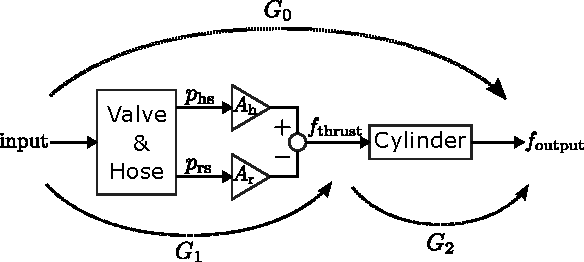
\includegraphics[keepaspectratio, scale=1.0]{contents/システム同定/figure/system_dentatsu.pdf}
        \caption{system}
        \label{fig:system_dentatsu}
\end{figure}

\subsection{線形性調査}
バルブへの入力に対するシステムの物理量の応答の線形性について調べ,システムの特性の把握を行う.
対象とする物理量は,実測出力$\fmsr$およびシリンダに取り付けてあるヘッド側圧力$\phs$,ロッド側圧力$\prs$である.

バルブへ正弦波入力を与えた際の応答をフーリエ変換し,そのピークが入力した正弦波の角速度と一致し,かつその他の角速度でピークが立たない場合に線形応答とみなすことができる.
実験では,バルブへ入力する角速度として\SI{0.1778}{rad/s}から\SI{100}{rad/s}まで対数上で等間隔に12等分したものを採用した.
サンプリング周期は\SI{0.001}{s}であり,センサから取得される値にはローパスフィルタ(以降LPF)として一次遅れの伝達関数${1}/(0.005s+1)$を通している.
また,直流成分をフーリエ変換を施す前に除去し,フーリエ変換後には角速度のピークに着目するため,最大ピークで除すことで正規化している.

各物理量の応答を\figname\ref{fig:1018FFT_fmeasure}から\figname\ref{fig:1018FFT_prs}に示す.
これより最大ピークの角速度と入力した正弦波の角速度が一致しているため,これらの物理量の応答は線形であるとみなすことができる.
よって対象とする油圧システムは線形なシステムとして扱い,同定することが可能である.
\begin{figure}[t]
    \centering
        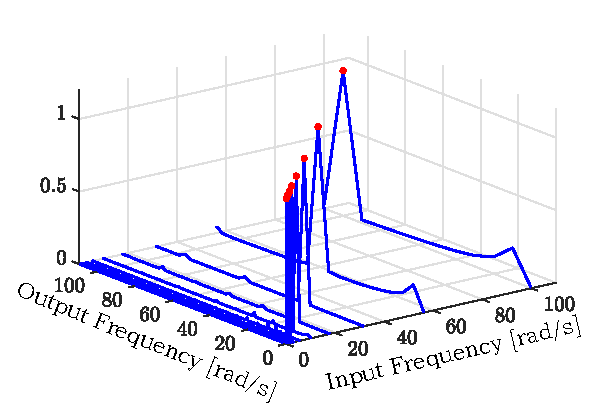
\includegraphics[keepaspectratio, scale=1.0]{contents/システム同定/figure/1018FFT_fmeasure.pdf}
        \caption{FFT of $\fmsr$}
        \label{fig:1018FFT_fmeasure}
\end{figure}
\begin{figure}[t]
    \centering
        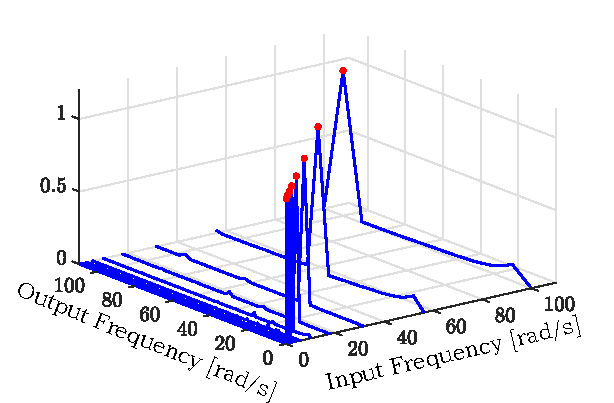
\includegraphics[keepaspectratio, scale=1.0]{contents/システム同定/figure/1018FFT_phs.pdf}
        \caption{FFT of $\phs$}
        \label{fig:1018FFT_phs}
\end{figure}
\begin{figure}[t]
    \centering
        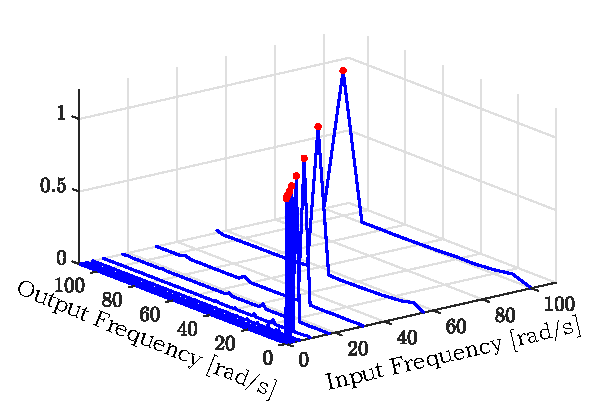
\includegraphics[keepaspectratio, scale=1.0]{contents/システム同定/figure/1018FFT_prs.pdf}
        \caption{FFT of $\prs$}
        \label{fig:1018FFT_prs}
\end{figure}


\subsection{周波数応答}
\subsection{最小自乗法による伝達関数モデルの同定}
\section{位置までの同定}
\subsection{線形性調査}
\subsection{周波数応答}
\section{M系列による同定}
\subsection{M系列の性質}
\subsection{システム同定(入力から位置)}
\subsection{システム同定(入力から力)}

